\problemname{Colourful Chameleons}

When Christian is not doing sophisticated research in software validation, he is breeding chameleons. His chameleons are of a special species and only occur in one of $n$ distinct colours. Unlike their counterparts in nature, Christian's chameleons change their colour only under very specific circumstances. It took Christian quite a long time to develop his so-called \textit{Crazy Chameleon Colouring Concept} ($C^4$) which works as follows. If he puts $n-1$ chameleons with distinct colours in a special breeding terrarium, gives them strawberry cheese and liver sausage to eat, and lets them stay in the dark over night, then there will be $y$ chameleons in the terrarium the next morning. The crazy thing is that none of the $y$ chameleons has any of the $n-1$ original colours. Instead, all of them take on the colour that was not present in the breeding terrarium initially.

Last weekend Christian let a friend borrow his chameleons for the Christopher Street Day. Of course his friend wanted the chameleons to look as colourful as possible. That's why Christian applied the $C^4$ method in a way such that there were at least $n-1$ chameleons available of every single colour. Therefore, Christian currently has $x_i \ge n-1$ chameleons of the $i$th colour. However, the next holiday coming up is St. Patrick's Day and Christian thinks that it would be super cool if all his chameleons took on the same colour for this special event. He is wondering whether such a state can be reached by exclusively applying the $C^4$ method. Because he is running low on strawberry cheese, he would like to know the minimal number of $C^4$ applications needed for all his chameleons to take on the same colour - provided that this is even possible.

\section*{Input}
The input consists of:
\begin{itemize}
	\item A line with three integers $n$, $c$, and $y$:
	\begin{itemize}
		\item $n$ ($2 \le n \le 10^5$), the number different colours that the Chameleons can take on.
		\item $c$ ($1 \le c \le n$), the colour that all chameleons should have in the end.
		\item $y$ ($n-1 \le y \le 10^9$), the number of chameleons in the breeding terrarium after applying the $C^4$ method.
	\end{itemize} 
	\item A line with $n$ integers $x_1,\ldots,x_n$ ($n-1 \le x_i \le 10^9$ for all $i$), where $x_i$ is the number of chameleons of the $i$th colour that Christian possesses initially.
\end{itemize}

\section*{Output}
If it is impossible for Christian's chameleons to all take on colour $c$ by exclusively applying the $C^4$ method, output \texttt{impossible}. Otherwise output two integer numbers $a$ and $b$, where $a$ is the minimal number of $C^4$ applications necessary for all chameleons to have colour $c$, and $b$ is the total number of chameleons that Christian possesses in the end.


\clearpage
\begin{figure}[!h]
	\centering
	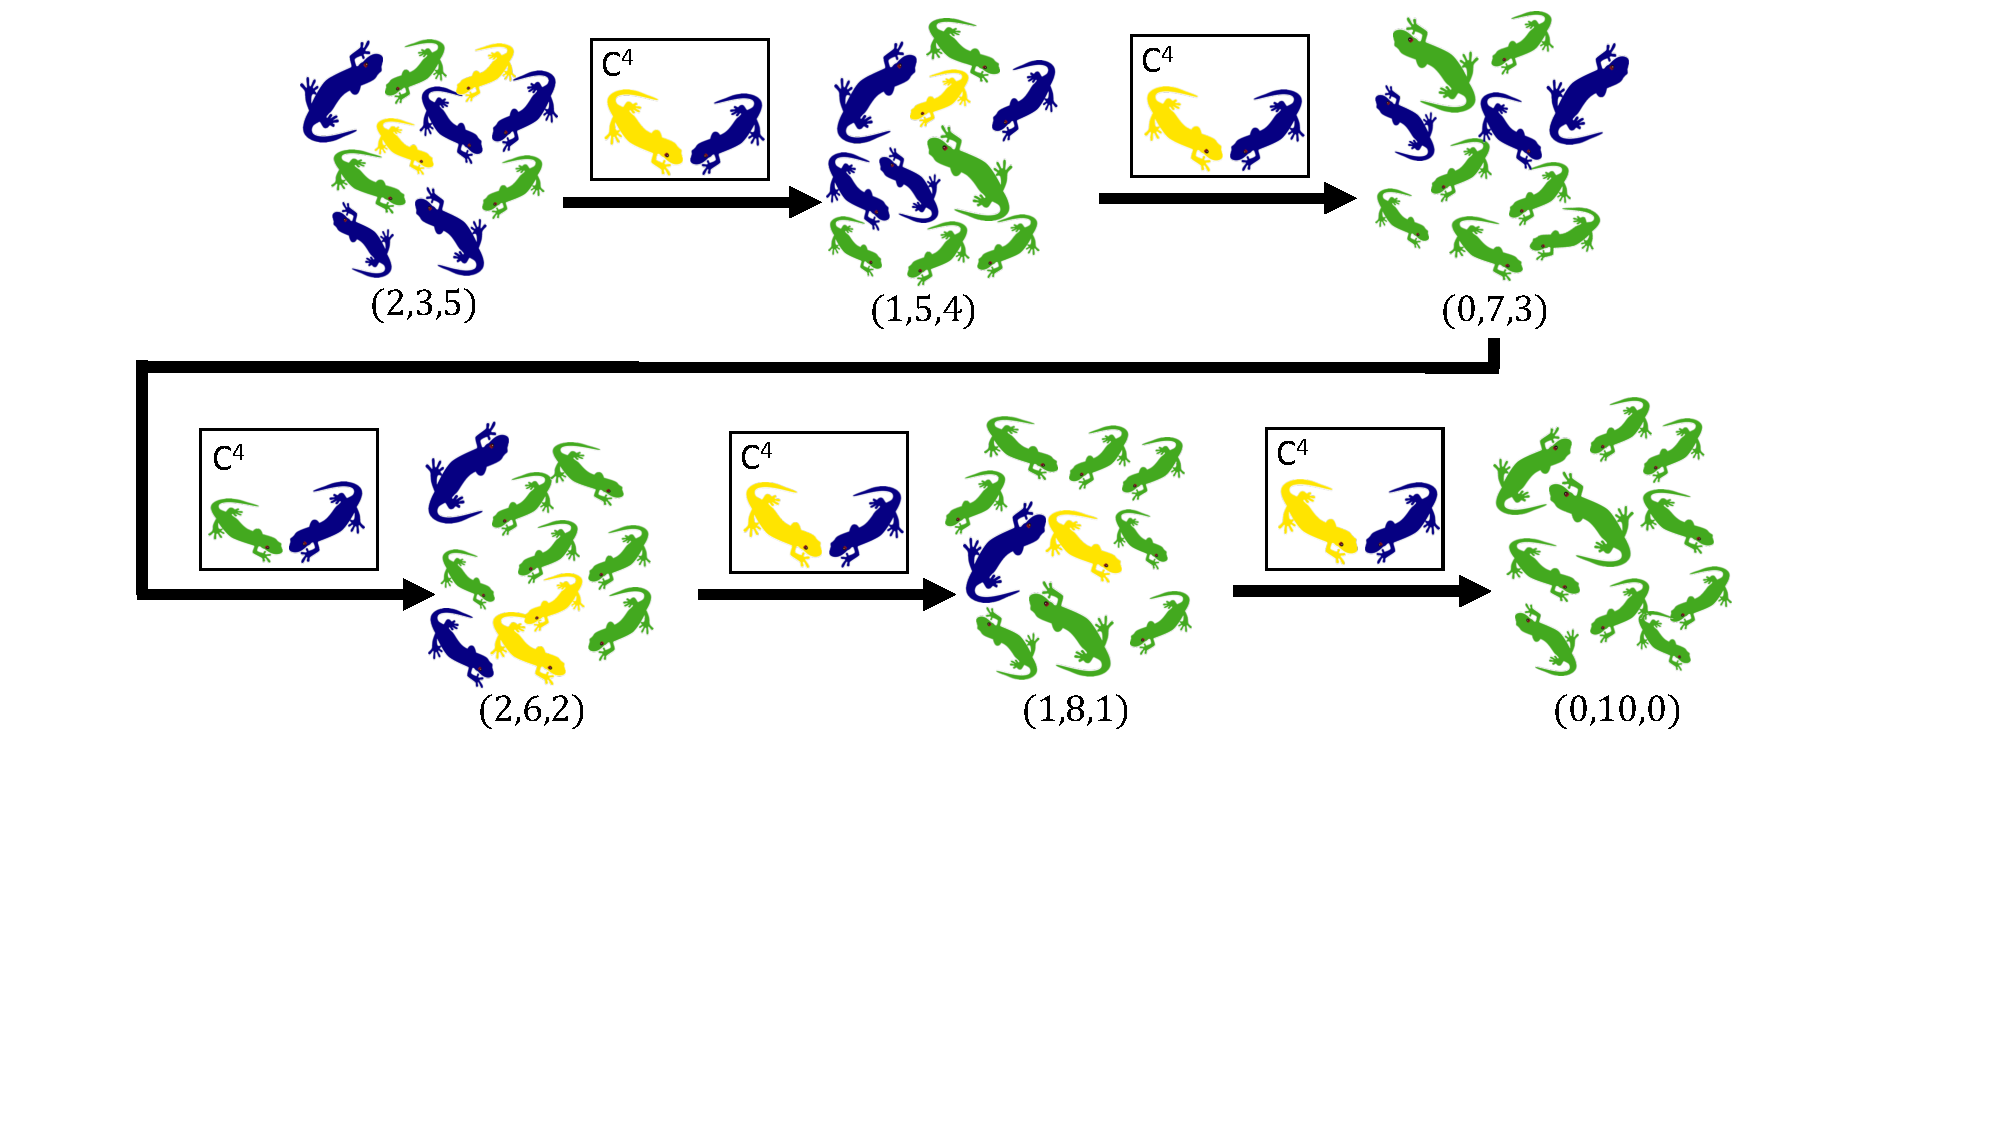
\includegraphics[width=\textwidth]{breeding.pdf}
	
	\vspace{2mm}
	\tiny{Images by \href{https://pixabay.com/de/vectors/eidechse-rot-bunte-reptil-kriecht-46815/}{OpenClipart-Vectors}
		on Pixabay.}
	
	\begin{minipage}{0.95\textwidth}
    \caption{Illustration of the first sample case. Initially, Christian owns 2 yellow, 3 green, and 5 blue chameleons. After 5 applications of the $C^4$ method he has 10 green chameleons. The vectors $(y,g,b)$ denote the number of yellow, green, and blue chameleons available in the respective breeding step.}
	\end{minipage}
\end{figure}
